\chapter{Optomechanical topology optimization problems}
%\section{Opto-mechanical systems~\cite{ownpub1,ownpub2,ownpub3}}\label{sec:optomechanics}
Optomechanics, the study of the interaction between light and mechanical motion, is at the heart of state-of-the-art technologies, such as 
optical trapping~\cite{ashkin_acceleration_1970, moffitt_recent_2008} and cooling~\cite{cooling}, quantum information processing~\cite{Andrews_2014, Xi_2025}
, light sails~\cite{lightsail, lightsail1}, and high-precision metrology and sensing~\cite{sensing, weakforce, Li:18, Mason_2019}. The most basic description of this interaction is given by the \textbf{Lorentz force}, which governs how moving charges respond to electric and magnetic fields:
\begin{equation}\label{eq:lorentz_f}
    \mathbf{\mathbf{F}}(\mathbf{r},t) = q \left[ \bm{\mathcal{E}}(\mathbf{r},t) + \mathbf{v}(t) \times \bm{\mathcal{B}}(\mathbf{r},t) \right]\,,
\end{equation}
where $q$ is the charge and $\mathbf{v}$ is the velocity of the particle. This force can be generalized to describe more complex systems,
such as the the force between two current-carrying 
wires (Ampere's force law), and the electromotive force, which is at the core of many techologies, such as induction motors or generators.
In optomechanical systems, shaping the distribution and magnitude of these forces at the micro- and nanoscale is crucial for controlling mechanical motion with light. 
However, designing structures that can efficiently harness and manipulate these interactions often requires navigating highly complex
 parameter spaces and trade-offs between optical, mechanical, and material constraints.

 One effective approach for enhancing and shaping optomechanical interactions is to use topology optimization.
Recent advances in optomechanical topology optimization include the design of coupling between optical and elastic
 waves~\cite{photo_topopt}, optical systems with nonlinear deformations~\cite{def_wg}, high-$Q$ optomechanical membranes~\cite{highQ1, fengwen, aragon1},
light sail structures~\cite{lightsail_topopt, lightsail_topopt1},
on-chip optical trapping devices~\cite{ownpub1}, particle design and manipulation~\cite{ownpub2, particle_opt},
and structural integrity constraint formulations~\cite{structural_integrity}
 among others.

 In the following subsections, we highlight our contributions to the field and review how to model optomechanical interactions in three distinct regimes: a general treatment based on the Maxwell stress tensor~\cite{ownpub2}; 
 the dipole approximation in the small particle limit~\cite{ownpub1, ownpub3}; and strongly coupled systems where optical forces can induce significant mechanical deformations.
\section{The Maxwell Stress Tensor formalism~\cite{ownpub2}}

In the most-general case, the optical force can be calculated using the \textbf{Maxwell stress tensor} (MST) formalism, which is a generalization of the Lorentz force (\eqref{eq:lorentz_f}) in continuous media~\cite{novotny}.
The basic idea is sketched in \figref{fig:eng_res}, where
a particle scatters an incident time-harmonic electromagnetic field $\mathbf{E}_\text{inc}$ creating the time-harmonic scattered field $\mathbf{E}_\text{scat}$ and the net force $\mathbf{F}$ that acts
on the particle. The time-averaged net force is given by~\cite{novotny}
\begin{equation}\label{eq:f_MST}
    \mathbf{F} \equiv \langle\mathbf{F}\rangle=\int_{\partial V}\langle\stackrel{\leftrightarrow}{\bm{\mathcal{T}}}(\mathbf{r}, t)\rangle \cdot \mathbf{n}_{\partial V}(\mathbf{r}) \d \mathbf{r}\,,
\end{equation}
where $\partial V$ denotes any boundary enclosing the particle, $n_{\partial V}$ denotes the unitary vector normal to that boundary, and
the time-average of the stress tensor is given by
\begin{equation}
        \langle \stackrel{\leftrightarrow}{\mathbf{T}}(\mathbf{r}, t) \rangle 
        = \frac{1}{2} \Re \Big\{ 
            \varepsilon\, \mathbf{E}(\mathbf{r}) \otimes \mathbf{E}^*(\mathbf{r})
            + \mu\, \mathbf{H}(\mathbf{r}) \otimes \mathbf{H}^*(\mathbf{r})
         - \frac{1}{2} \big( \varepsilon\, |\mathbf{E}(\mathbf{r})|^2 + \mu\, |\mathbf{H}(\mathbf{r})|^2 \big) 
        \stackrel{\leftrightarrow}{\mathbf{I}} \Big\}.
\end{equation}
where $\otimes$ denotes the outer product. Note that the permittivity ($\varepsilon$) and permeability ($\mu$) correspond to those of the medium surrounding the particle.

\begin{figure}[tb]
    \centering
    \makebox[\textwidth][c]{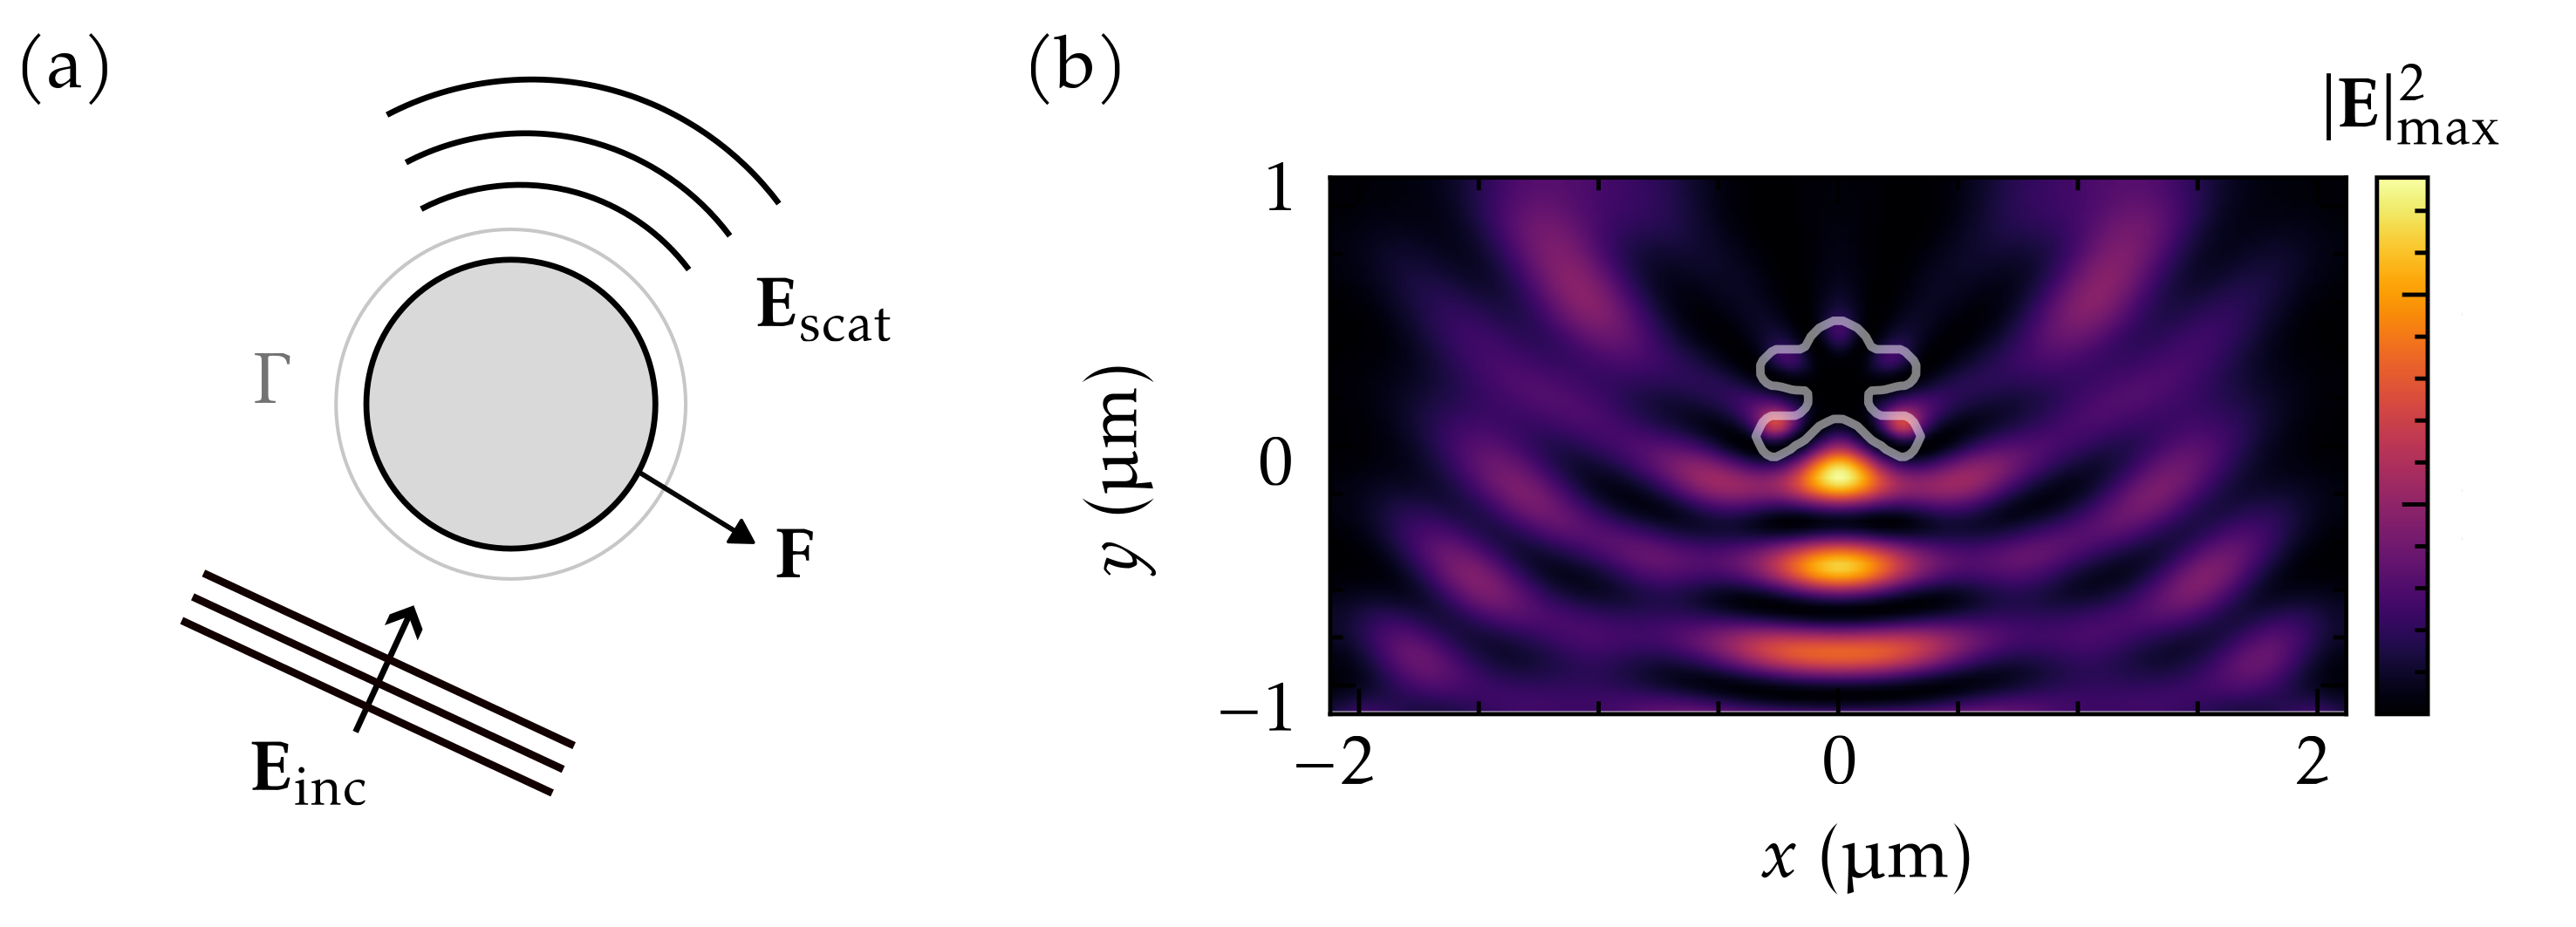
\includegraphics{figures/eng_results.png}}%%
    \caption{Topology optimization in optical force applications. (a) A scattering particle 
    enclosed by a boundary $\partial V$ scatters a field $\mathbf{E}_\text{scat}$, when excited by an incident field $\mathbf{E}_\text{inc}$, 
    generating a net optical force $\mathbf{F}$. (b) Electric-field intensity distribution for a particle design optimized to maximize the vertical ($y$)
    component of the optical force. Adapted with permission from~\cite{ownpub2} \copyright Optical Society of America.}
    \label{fig:eng_res}
\end{figure}

\subsection*{Engineering optical forces via topology optimization}

In~\cite{ownpub2} we apply this formalism to optimize the geometry of particle-metalens pairs for difference applications, such as attracting, repelling, 
oscillating and trapping particles. In \figref{fig:eng_res} we depict an example optimization result from our work, where 
we optimize the geometry of a particle to maximize the vertical component of the optical force by targeting $\text{FOM} = \langle\mathbf{F}\rangle \cdot \mathbf{n}_y$, where
in our two-dimensional example $\mathbf{n}_y = (0, 1)$ is the unitary vector in the vertical direction.  Our results show that the optimized particle geometry is a Bragg-mirror-like
structure, which is able to efficiently reflecting the incoming plane-wave, resulting in a efficient exchange of force and momentum. As a matter of fact, by comparing the response of the optimized design
to a reference square particle, we observe that the topology-optimized device feels a $\approx 3\times$ stronger vertical force than the reference.
 Moreover, in~\cite{ownpub2} we show that by also designing a metalens to focus the incoming plane-wave onto the particle one can use nearly all the momentum available in the simulation domain\footnote{This is based on the radiation pressure force on an perfectly reflecting surface spanning the entire simulation domain~\cite{ownpub2}.} 
 to generate a net force on the particle, allowing for a $\approx 13\times$ stronger force than the reference square particle. 
 In the remainder of~\cite{ownpub2} we further extend these examples by also designing
attractive particle geometries, and optical-tweezer like setups to trap the particle in space. All the code developed in this work is available on GitHub~\cite{github_MST} with tutorials on force calculation and topology optimization. 

One interesting aspect of the topology optimization of particles in the MST formalism is that with our current framework the particle cannot feature disconnected members; otherwise,
one would need to integrate around the individual components to calculate the total force for each one. It is possible solving this problem by enforcing 
a connectivity constraint via the VTM~\cite{li_structural_2016} (see \secref{sec:aux}). In our examples
we enforce particle connectivity to the center of the particle, and connect the metalens structure to the bottom, as to ensure structural
integrity of the structure.

\subsection*{Outlook and future work}

This topology optimization work is the first, to our knowledge, to 
target optical forces via the MST formalism, paving the way for future work in three-dimensional systems and more complex optimization problems, such as optically-driven particle
trajectory control~\cite{zemanek_perspective_2019, macdonald_microfluidic_2003, shilkin_directional_2017}, many-body particle systems~\cite{bechinger_active_2016, chang_colloquium_2018} or optically actuated devices~\cite{ivanyi_optically_2024}, among others.
Finally, it is worth noting that a particularly interesting and straightforward extension of the framework would be to use the MST formalism to calculate the time-averaged torque acting on a particle, defined as~\cite{novotny}
\begin{equation}
    \langle \bm{\tau} \rangle = \langle \mathbf{r} \times \mathbf{F} \rangle = \int_{\partial V} \langle \mathbf{r}
     \times \stackrel{\leftrightarrow}{\bm{\mathcal{T}}} \rangle \cdot \mathbf{n}_{\partial V} \d\mathbf{r} 
\end{equation}
where $\mathbf{r}$ is the vector defimed between the rotation axis and force application point. This definition of torque accounts
for two kinds of rotational motion; \textit{spinning} ($\langle \bm{\tau}_S \rangle$), where the particle rotates around its center of mass,
and \textit{orbiting} ($\langle \bm{\tau}_O \rangle$), where the particle rotates around an external axis, so that the total torque is the sum
of both the spin and orbital torque $\langle \bm{\tau} \rangle = \langle \bm{\tau}_S \rangle + \langle \bm{\tau}_O \rangle$~\cite{torque}.  Defining
and optical torque-based FOM could open the door for the design of efficient optical and biological micro- and nanomachines~\cite{rotating, gluck}.

\section{The dipole approximation~\cite{ownpub1, ownpub3}}

When particles are much smaller than the wavelength of the electromagnetic field ($s\ll \lambda$), it is possible to model the optical force via the dipole approximation in the
quasistatic limit (see \secref{sec:nanophotonics}). In this approximation, the particle is treated as a point dipole with a polarizability $\alpha$, which describes how the particle responds to the local electric field frequency-domain $\mathbf{E}$.
In the dipole approximation the optical force on the particle can be expressed as~\cite{novotny}:
\begin{equation}\label{eq:dip_force}
    \langle\mathbf{F}\rangle=\overbrace{\frac{\alpha^{\prime}}{4} \nabla\left\{\mathbf{E}^* \cdot \mathbf{E}\right\}}^{(\text{G})}
    +\frac{\alpha^{\prime \prime}}{k \varepsilon_0} \Big[\overbrace{\frac{1}{c}\langle \mathbf{S} \rangle}^{(\text{RP})} + \overbrace{c \left( \nabla \times \langle \mathbf{L} \rangle \right)}^{(\text{SC})}\Big]\,,
\end{equation}
where the polarizability can be split up into the real and imaginary parts 
$\alpha=\alpha^\prime + i \alpha^{\prime \prime}$, the Poynting vector is given by $\mathbf{S} = \mathbf{E} \times \mathbf{H}$, and the time-averaged angular momentum is 
$\langle \mathbf{L} \rangle = [\varepsilon_0/(4 i \omega)](\mathbf{E} \times \mathbf{E}^*)$. 
The term associated with the electric field intensity (G) is \textbf{gradient force}, the term with the Poynting vector is the radiation pressure (RP), while the term associated 
with the angular momentum (SC) is the spin-curl force.

In the abscence of absorption effects ($\alpha^{\prime \prime}=0$), the force is totally described 
by the gradient force, which is a conservative force that can be described as the gradient 
of a potential:
\begin{equation*}
    U (\mathbf{r}) = -\frac{\alpha^{\prime}}{4} \left|\mathbf{E}(\mathbf{r})\right|^2\,.
\end{equation*}
where the force can be calculated as $\mathbf{F} = -\nabla U(\mathbf{r})$. In optical trapping applications $U$ is often referref to as the \textbf{trapping potential}.
For non-resonant and non-absorbing isotropic particles the polarizability is 
described through the relation~\cite{BornWolf:1999:Book} 
    $\alpha^{\prime}= 3 \varepsilon_0 $V$ (\varepsilon_p-\varepsilon_m)/(\varepsilon_p+2 \varepsilon_m)\,,$
where $V$ is the volume of the particle, $\varepsilon_p$ and $\varepsilon_m$ are the
dielectric constants of the particle and the medium, respectively. Note that in the dipole approximation, for infinitesimally small particles, the field $\mathbf{E}$ is not modified by the presence of the particle.
This works well for point-like particles in free-space but not necessarily 
for either large particles, particles with high refractive contrast, or particles close to material
boundaries (e.g., optical cavities). The interaction between the background field and the particle interaction can be accounted for in the dipole
approximation by considering the \textbf{self-induced back-action} (SIBA) effect, which assumes a weak
perturbation of the field due to the presence of the particle and expands the field in terms of 
the scattering Green function of the particle, which leads to a self-consistent
equation for the total electric field which can be used to calculate the force~\cite{novotny, SIBA, benjamin}. If the series converges this leads 
to same result as the MST calculation (\eqref{eq:f_MST}), which is often used to validate the dipole approximation (e.g., \cite{ownpub1,ownpub3}). 

\subsection*{On-chip omnidirectional optical trapping via topology optimization~\cite{ownpub1}}

Using the dipole approximation formalism in~\cite{ownpub1} we use topology optimization to design an integrated omnidirectional trapping optical cavity,
which was previously only possible with the use of free-space optical tweezers~\cite{ashkin_acceleration_1970}, or bulky photonic devices~\cite{manka_simulation_2024}. The trapping device
consists of two silicon waveguides connected to a central design domain, in which
topology optimization is applied (\figref{fig:MST_dipole}). The central region contains a cylindrical air exclusion with a radius
$R_\text{exc}=300$ nm and a thickness of $800$ nm, in which the stable trap is located.
To design an omnidirectional trapping device we minimize  
the difference of the electric-field norm with respect to a reference field $\mathbf{E}_\text{ref}$:
\begin{equation}
    \text{FOM} \equiv \Phi=\sqrt{\int_{\Omega}\left[\Theta_{\beta,\eta}\left(\frac{|\mathbf{E}(\mathbf{r})|}{\left|\mathbf{E}\left(\mathbf{r}_0\right)\right|}-\frac{\left|\mathbf{E}_{\text{ref}}(\mathbf{r})\right|}{\left|\mathbf{E}_{\text{ref}}\left(\mathbf{r}_0\right)\right|}\right)\right]^2} \text{~d} \Omega
    \end{equation}
where the fields are normalized with respect to the value at the center of the cavity ($\mathbf{r}_0$), and $\Theta_{\beta,\eta}$ is the smoothed Heaviside threshold (\eqref{eq:threshold}), which ensures
potentials as steep or steeper than the reference. The reference is chosen as a Gaussian trapping potential with standard deviations $\sigma_x=\sigma_y=300$ nm and $\sigma_z=400$ nm, but can be chosen to have any other form, such as a harmonic potential ($U\propto\mathbf{r}^2$).

By applying this optimization framework we obtain the topology-optimized cavity design in \figref{fig:MST_dipole}, which is able to trap particles at the center of an optical
cavity in three dimensions and has an associated Gaussian-like trapping potential, with a depth  $U<-10\, k_B T$ at room temperature ($T=300$ K) conventionally needed to overcome Brownian fluctuations~\cite{novotny}.
Note that one of the strengths of this framework is that it relies on the dipole approximation, so that
as long as the dipole approximation is valid, one can tune the input power to trap paricles of arbitrarily small sizes.

\begin{figure}[tb]
    \centering
    \makebox[\textwidth][c]{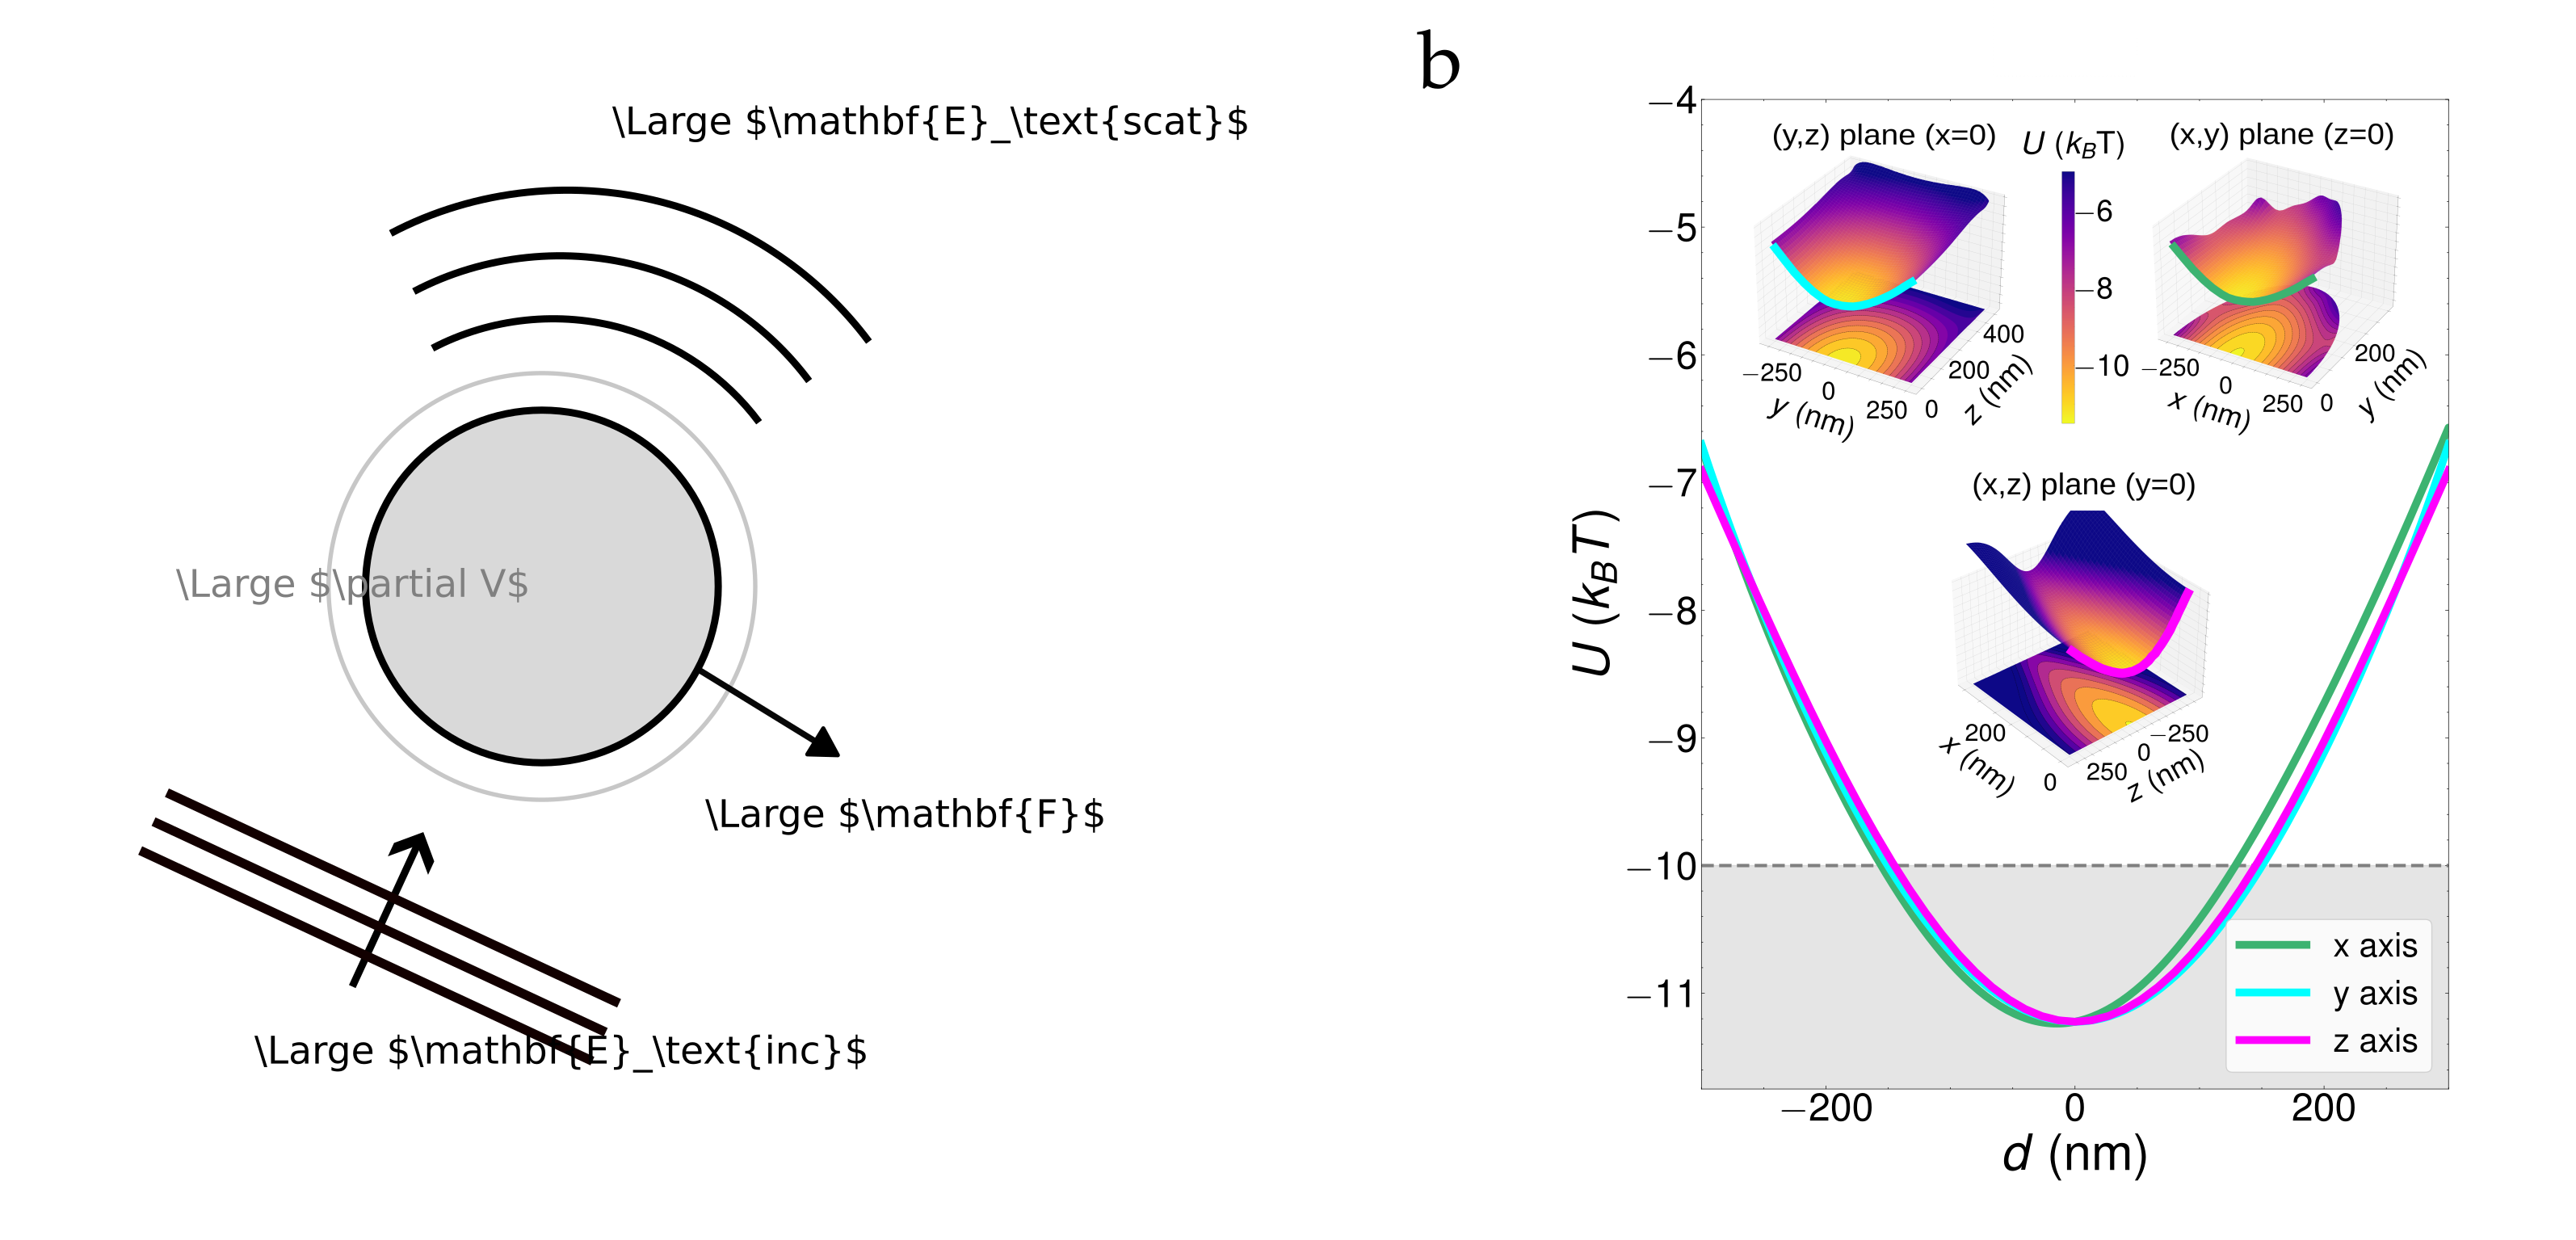
\includegraphics{figures/MST_dipole.png}}%%
    \caption{Optical response and trappig potential for the topology-optimized particle trap. (a) Lower half ($z<0$) of the optimized cavity, with the electric-field intensity
    distribution when excited with the fundamental waveguide mode at $\lambda=1.55$ \textmu m. (b) Trapping potential for a $R=15$ nm and $n=2$ particle in the cavity region for the different axial line- and plane-cuts as a function
    of the distance from the center ($d$), with the stable trapping regime ($U<-10 k_B\, T$) highlighted in gray. Adapted with permission from~\cite{ownpub1}.}
    \label{fig:MST_dipole}
\end{figure}

From the dipole approximation trapping potential we calculate the the force-displacements curves and we determine trapping stiffnesses
of $\kappa \approx 0.5$ fN/nm, an order of magnitude larger that diffraction-limited free-space optical tweezers~\cite{ownpub1}. To validate this findings
we employ the MST formalism to calculate the force on spherical particles as they are displaced from the cavity center and find excellent
agreement with the dipole approximation. As shown in \figref{fig:SPIE}, to further verify the the dipole approximation assumption, in~\cite{ownpub3} we compare the results of the dipole approximation with the MST
for varying spherical particle radii ($R_\text{sph}$) and refractive indices ($n_\text{sph}$), showing good agreement between the two methods
even for large values of the refractive index (e.g., $n_\text{sph}=3$) and particle sizes up to $s \sim R_\text{sph}\approx 0.05 \lambda$.
\begin{figure}[tb]
    \centering
    \makebox[\textwidth][c]{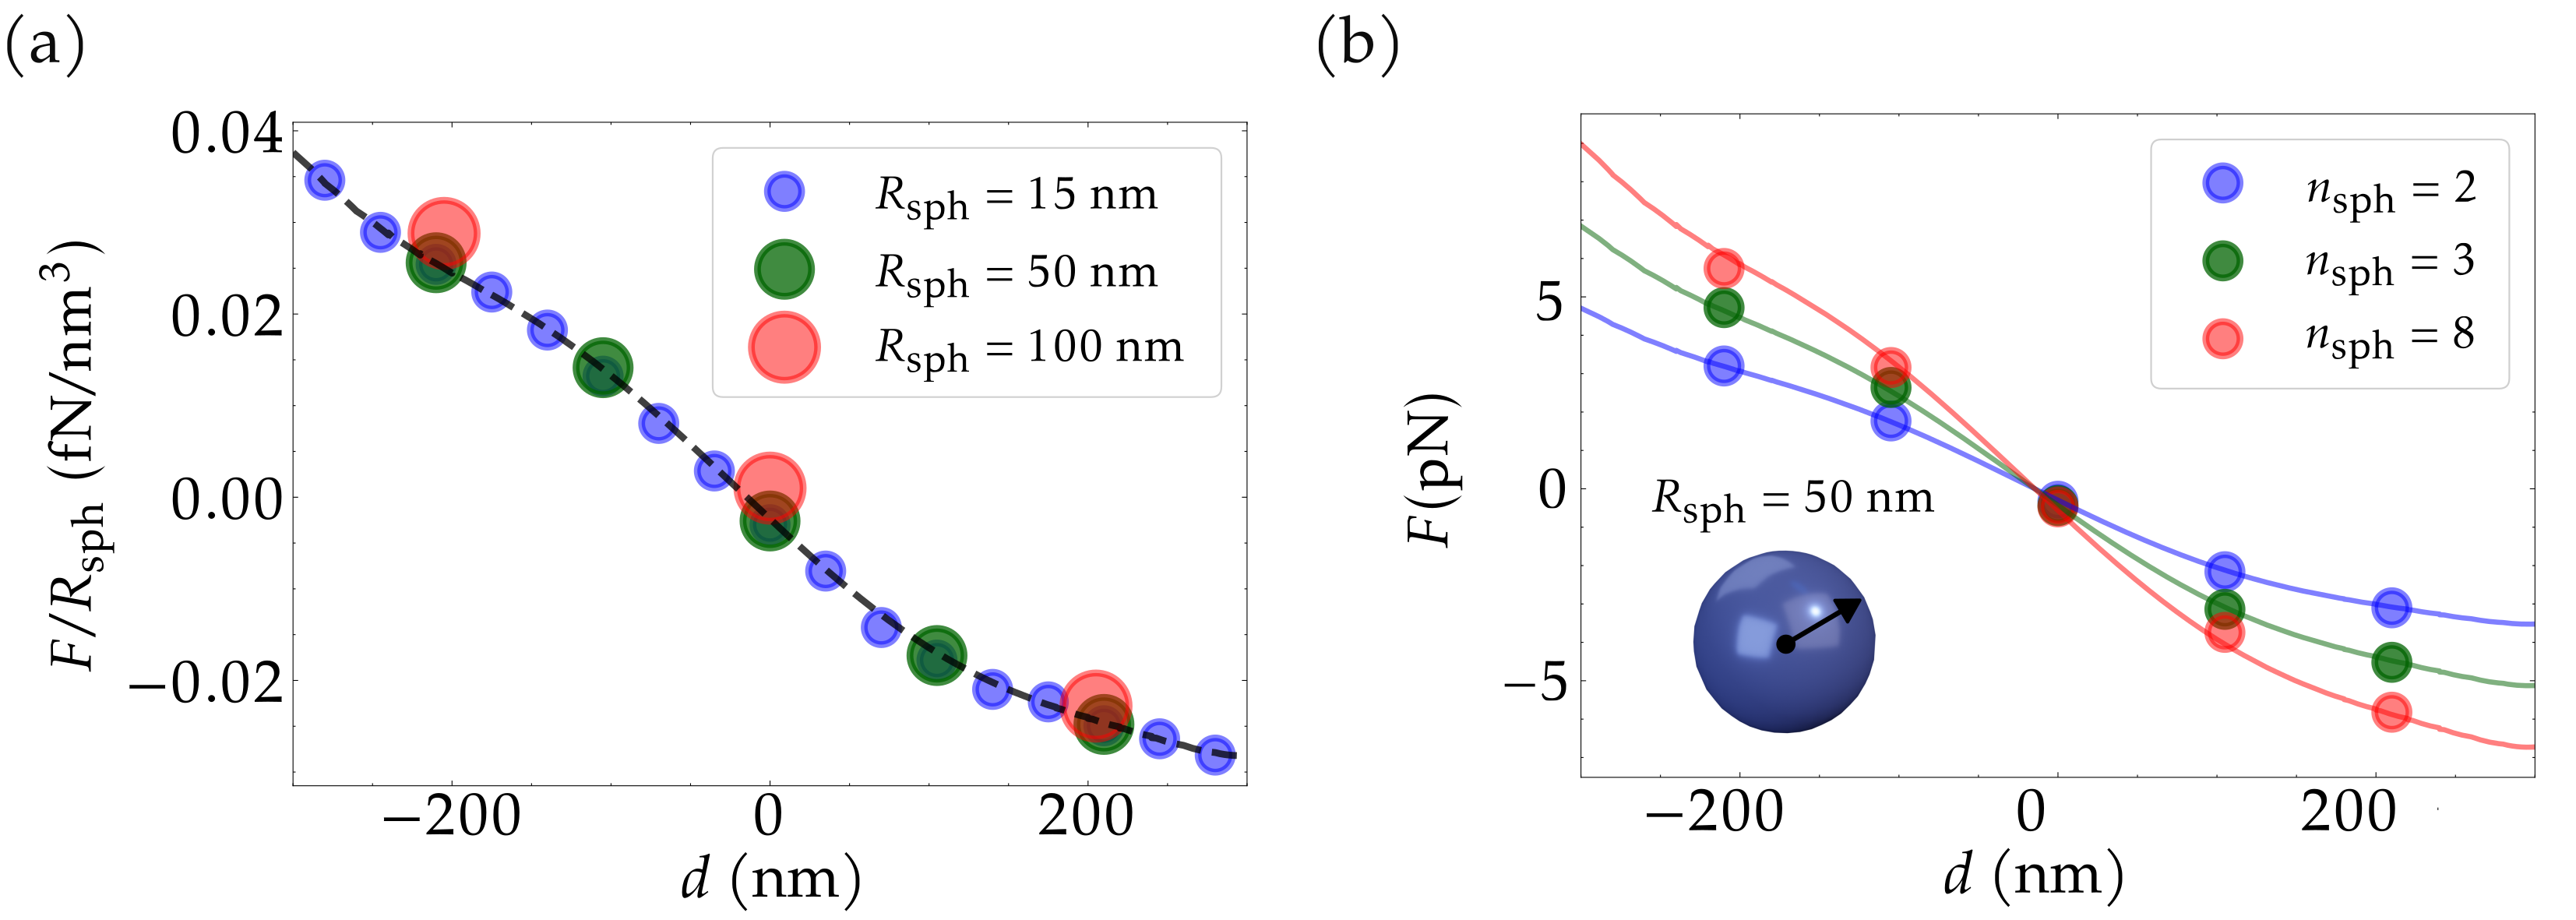
\includegraphics{figures/SPIE_results.png}}%%
    \caption{Validating the dipole approximation force (dashed line) against the MST force (data points), for the force as a function of displacement ($d$) from the cavity center.
    (a) Volume-normalized force ($F/R^3_\text{sph}$) for different particle sizes with refractive index $n_\text{sph}=2$. (b) Force for different refractive indices of the particle for a particle radius $R_\text{sph}=50$ nm. Adapted from~\cite{ownpub3}.}
    \label{fig:SPIE}
\end{figure}

\subsection*{A metric for trapping performance~\cite{ownpub1}}

When designing optical trapping platforms it is important to be able to compare performance across platforms. To this end, in~\cite{ownpub3} we introduce a normalized
trapping stiffness metric, which normalizes trapping stiffness to particle  polarizability and input power ($P_\text{in}$)
\begin{equation}
    \eta_i=\frac{\kappa_i \varepsilon_0}{\alpha^\prime P_{\text{in}}}
\end{equation}
enabling one-to-one comparison across trapping devices\footnote{As noted in~\cite{ownpub3} this metrics breaks down for lightless platforms (e.g., Casimir force-based traps), and the metric could be redefined
without including the input power.}. The normalized trapping stiffness allows us to show that (Tab. 1 in~\cite{ownpub3}), although plasmonic devices can reach higher normalized 
stiffnesses, they suffer from optical losses to heating and lack omnidirectional stable trapping. In contrast, the inverse-designed dielectric platform in \figref{MST_dipole}
 achieves comparable normalized stiffnesses to other dielectric traps while uniquely offering fully stable, omnidirectional trapping
  without relying on SIBA effects. Notably, SIBA-based devices are particle-specific and their performance can break down
   for different particle geometries or materials. Compared to conventional optical tweezers, our device maintains similar trapping
    strength at lower input power due to its integrated, waveguide-coupled design, highlighting the benefits of miniaturized,
     near-field-based optical trapping.

\subsection*{Outlook and future work}

Aside from the results presented here, in~\cite{ownpub2} we discuss the effects of Casimir-Polder effects
 on particle loading and outline potential applications of our proposed devices in particle optomechanics
  and biophotonics, where compact, integrated, omnidirectional trapping could
   enable new technologies. The demonstrated trapping concept shows promise for applications in biophotonics, and fundamental physics,
    offering strong confinement with low input power for deeply sub-wavelength particles.

Future work could focus on extending the inverse design framework to support alternative materials, 
traps for lossy or resonant particles, and devices with multiple trapping sites.
 Such developments could enable scalable arrays of trapped quantum emitters, with potential applications
  in quantum optics and many-body physics~\cite{chang_colloquium_2018}. We anticipate that experimental demonstrations
   will validate these predictions and push the limits of integrated omnidirectional trapping.

\section{Strongly coupled optomechanical systems}\label{sec:mech_strongly_coupled}

In strongly coupled optomechanical systems, the optical field can significantly modify the mechanical properties of the system, leading to a significant deformation
of the device, which in turn modifies the optical response. In most optomechanical systems the optical response is much faster than the mechanical response, since the 
mechanical frequencies ($\omega_\text{mech}$) are orders of magnitude lower than the optical frequency ($\omega_\text{mech}\ll\omega$) or optical resonance decay rates ($\omega_\text{mech}\ll\kappa$, so one 
can neglect sideband cooling or amplification)\cite{opto_crys, photo_topopt}(cite). Due to the slower mechanical dynamics, it is possible to analyze the mechanical response of the structure in the quasistatic approximation, by only considering the mechanical steady-state response of the structure. 
This can be accounted for by considering the time-averaged force in the MST formalism (\eqref{eq:f_MST}) the local steady-state
force balance equation:
\begin{equation}
    \nabla \cdot \overleftrightarrow{\boldsymbol{\sigma}} = \mathbf{f}_\text{MST}  \,,
\end{equation}
where the volumetric force from the MST is given by $ \mathbf{f}_\text{MST} = \nabla \cdot \langle \stackrel{\leftrightarrow}{\bm{\mathcal{T}}} \rangle$ and $\overleftrightarrow{\boldsymbol{\sigma}}$ is the stress tensor of the mechanical system. Solving for the mechanical
displacement $\mathbf{u}$ [e.g., via the finite element method (\secref{sec:fem})], one can then calculate the mechanical deformation of the system, which together with the solution to the optical problem
(\eqref{eq:wave_eq}) consitutes the basics to solve a strongly coupled optomechanical probelm. In the next section, we highlight some key results of our unpublished work, where we apply this formalism to the 
topology optimization of an optomechanical membrane-like device.

\subsection*{Topology optimization of strongly coupled optomechanical membranes}

To exemplify the use of topology optimization in the context of strongly coupled optomechanical problems we consider the example of the two-dimensional representation of an optomechanical membrane-like device, which
is based on a clamped-clamped beam attached to a central design domain (see Fig. 1 in ). The device is excited by an incoming plane-wave from the bottom, which will generate a mechanical volumetric load on the structure ($\mathbf{f}_\text{MST}$)
which will deform the structure upwards. The goal of the optimization problem is to maximize the vertical component of the displacement at a point ($\mathbf{r}_0$)
in the structure.

We solve the strongly coupled optomechanical by considering an optical frequency-domain problem coupled to a geometrically nonlinear mechanical problem. Discretizing the system via the finite element
method gives the coupled system of equations
\begin{equation}\label{eq:coupled}
    \begin{aligned}
        \mathbf{S}\left(\alpha\mathbf{U}\right) \mathbf{E} &= \mathbf{E}_\text{in} , \\
        \mathbf{R}[\mathbf{U}, \langle \mathbf{F}_\text{MST}(\mathbf{E})\rangle] &=\mathbf{0}\,,
    \end{aligned}
    \end{equation}
where $\mathbf{S}$ is the discretized system matrix which encodes the operators
 in the optical problem, $\mathbf{E}$ and 
 $\mathbf{E}_\text{in}$ are the vectors containing the nodal degrees-of-freedom for the electric 
field and the forcing term respectively; $\mathbf{R}$ is the residual of the
 geometrically nonlinear mechanical problem~\cite{cook_concepts_2001}, and 
 $\mathbf{U}$ and $\mathbf{F}_\text{MST}$ are the vectors containing the nodal
  degrees-of-freedom for the displacement field and the MST forcing term respectively. 
  Moreover, we consider the parameter $\alpha$, which allows us to control if we consider 
  the strongly coupled problem ($\alpha=1$), where the optical field deforms the structure, 
  or the weakly coupled problem ($\alpha=0$), which is a good approximation in the small deformation 
  limit ($\alpha\mathbf{U} \ll 1$). To solve the strongly coupled problem in 
  \eqref{eq:coupled} we use a seggregated scheme (see Fig. 2 in ), where the
   mehcanical solution is applied to the geometry via a mesh deformation, and
    both problems are solved until a convergence criteorion is fullfilled.

    For the topology optimization we consider a linear material interpolation for the Young's modulus\footnote{We did not experience any problems with grayscale in this problem, so we did not use the standard power-law penalization~\cite{SIMP}.} and the 
    refractive index. More importantly, to introduce the optical force loads in our mechanical problem, one would need to identify the boundaries of the design according to \eqref{eq:f_MST}. However, in density-based topology optimization problems boundaries
     are not well defined in the design process and it can sometimes be cumbersome to find and detect boundaries when having intermediate density values while solving the optimization problem~\cite{jdara}. To circumvent this issue, we apply Gauss' theorem to
      redefine a volumetric mechanical load on the structure that is linearly proportional to the physical design field
    \begin{equation}
    \langle\mathbf{f}_\text{MST}\rangle= \hat{\rho} \int_{\Omega} \nabla \cdot \langle\overleftrightarrow{\mathbf{T}}(\mathbf{r}, t)\rangle \d \Omega\,,
    \end{equation}
    where $V$ is the volume where the force is acting upon. Lastly, to ensure structural integrity we applu a connectivity constraint via the VTM~\cite{li_structural_2016} (see \secref{sec:aux}), which ensures that the design is connected to nanobeams. 


\begin{figure}[tb]
    \centering
    \makebox[\textwidth][c]{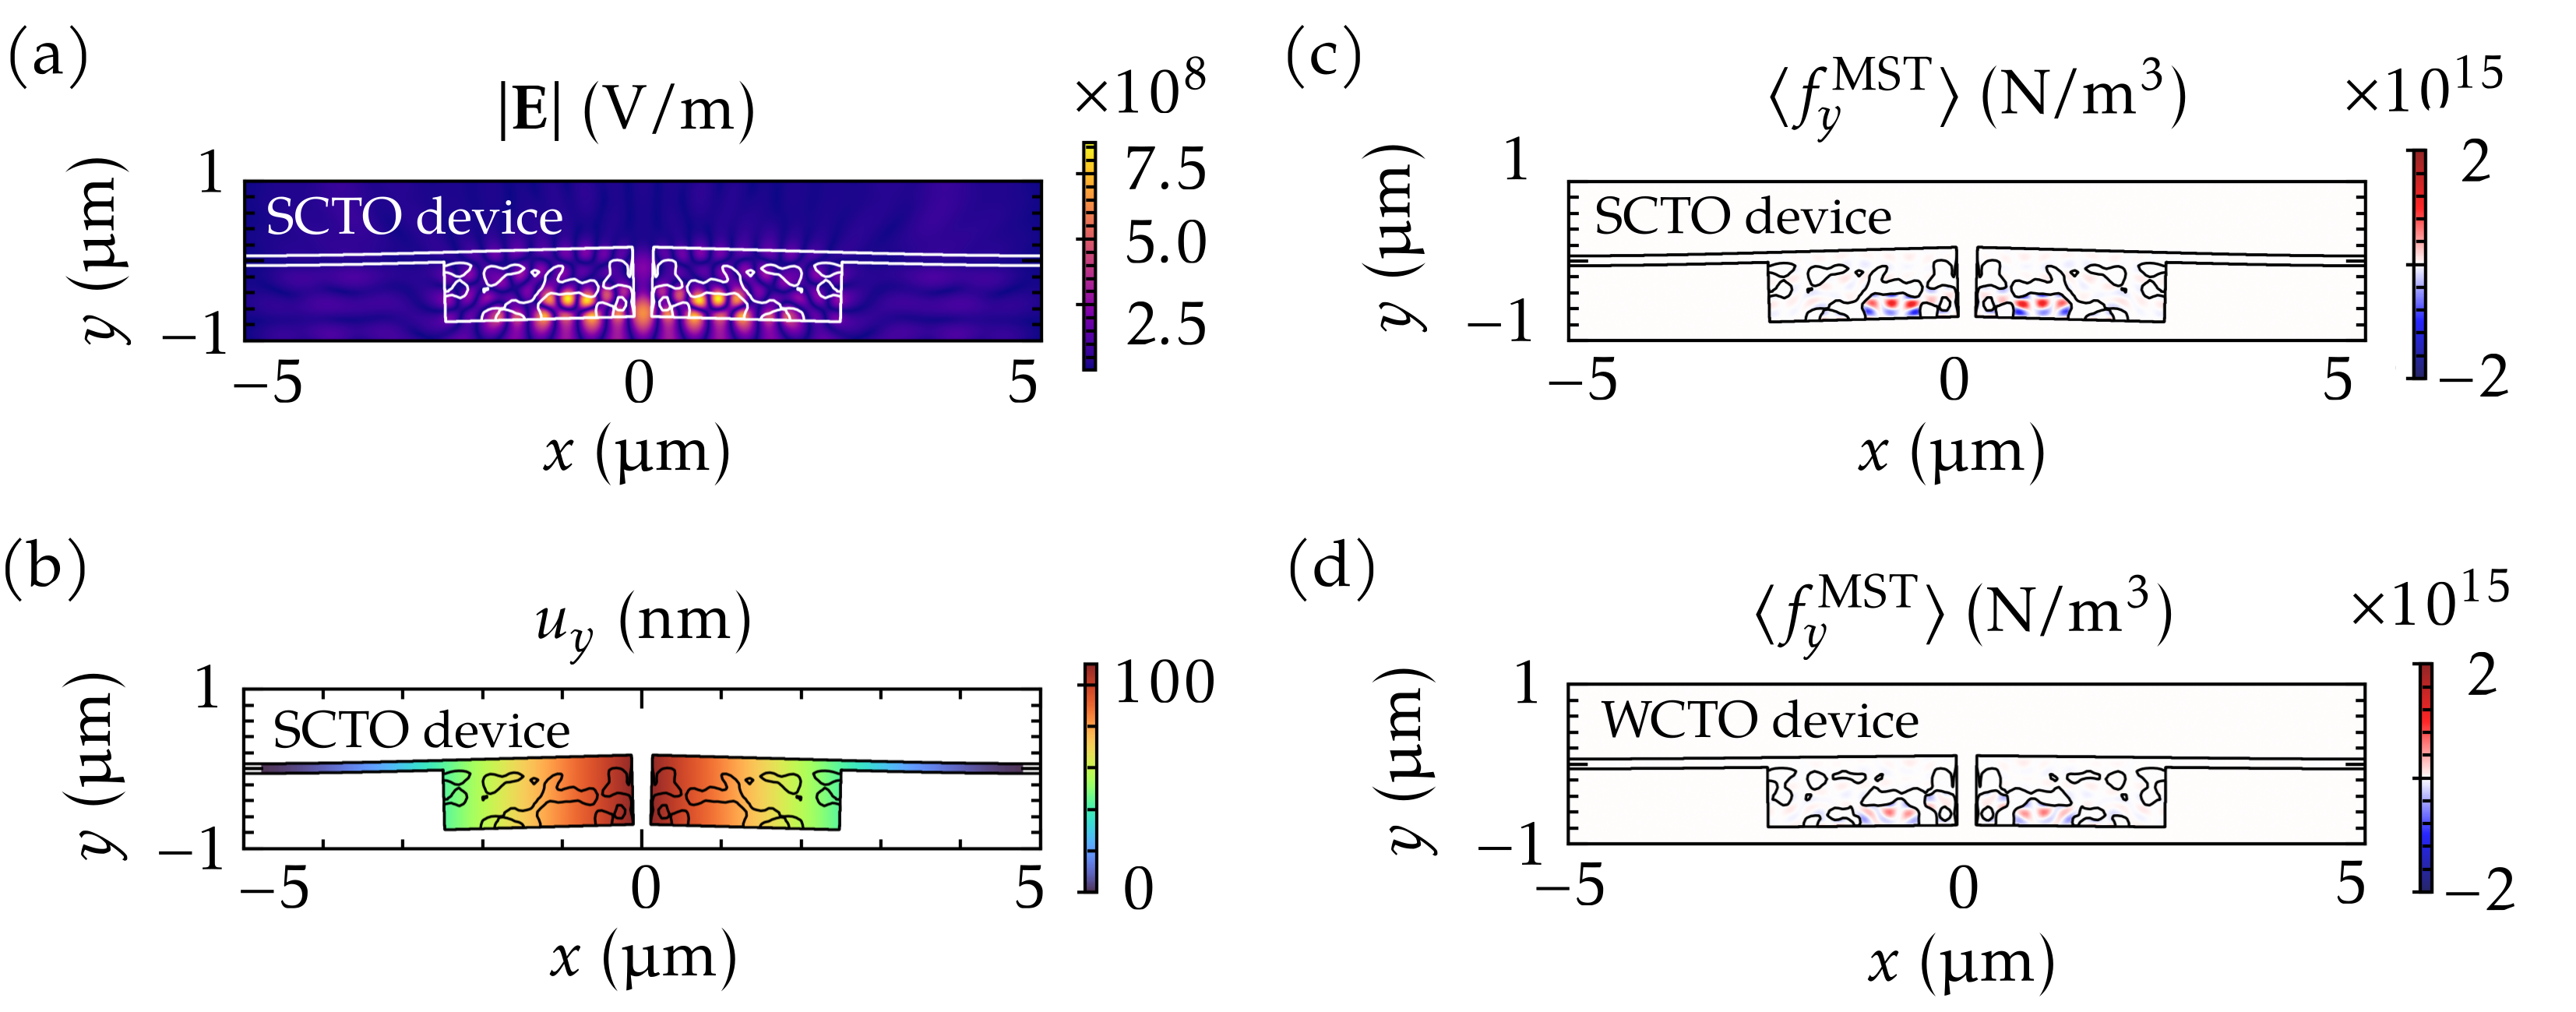
\includegraphics{figures/fields_panels_SC.png}}%%
    \caption{Device evaluation in the deformed material configuration. (a) Electric-field norm ($\vert\mathbf{E}\vert$) for the SCTO device. (b) Vertical ($y$) component of the MST force ($\langle f^\text{MST}_y\rangle$) for the SCTO device. (c) Vertical ($y$) component of the MST force ($\langle f^\text{MST}_y\rangle$) for the WCTO device. (d) Vertical displacement ($u_y$) for the SCTO device.}
    \label{fig:SC}
\end{figure}


    Using this formalism we solve the topology optimization for a membrane-like device that has a hole in the center of the design region (FORMULATE BETTER) and find
    the results in \figref{fig:SC}, for the SCTO (optimized for strong coupling, $\alpha = 1$) and WCTO (optimized for weak coupling, $\alpha = 0$) devices.
    When evaluated with the fully coupled model, the SCTO device achieves a figure of merit (FOM) of about 110\,nm, while the WCTO reaches only about
     43\,nm, demonstrating a $\sim$3$\times$ improvement when the full coupling
      is included during optimization. Evaluating the WCTO under the
       weakly coupled model gives an FOM of $\sim$69\,nm, highlighting
        a significant drop due to neglecting coupling effects in the design. 
        The improved performance of the SCTO stems from its asymmetric structure, which breaks symmetry,
         induces rotation, and produces heterogeneous vertical displacements that more strongly modulate 
         the optical force distribution, resulting in tilted, Bragg-mirror-like features that more effectively reflect the incoming field.

\subsection*{Outlook and future work}

This topology optimization framework can be readily applied to a wide
 range of optomechanical devices and paves the way for future developments. 
 For example, extending the method to include clamping losses and three-dimensional designs
  would improve accuracy for high aspect-ratio membranes, while adding
   photoelastic effects would capture strain-induced refractive index changes.
    The framework also holds promise for cavity optomechanics beyond the quasistatic
     regime by replacing steady-state models with frequency-domain solvers. 
     Moreover, incorporating models like third-medium contact could enable the design of
      flexible or reconfigurable systems where large deformations and mechanical nonlinearities
       strongly affect optical performance. ADD CITATIONS

